%start by defining the document class
\documentclass[12pt]{article}

%below the package used for hyperlinking
\usepackage[a4paper, top=2.3cm, bottom=2.3cm, left=2.3cm, right=2.3cm]{geometry}
\usepackage{graphicx}	
\usepackage[brazil]{babel}
\usepackage{float}
\usepackage{hyperref}
\usepackage{amsfonts} 
\usepackage{amsmath}
\usepackage[brazil]{babel}
\graphicspath{ {images/} }

\linespread{1.5}
\setlength{\parindent}{1.3cm}

\begin{document}

\begin{titlepage}
    \begin{center}
        \vspace*{1cm}
            
        \Huge
        \textbf{Simulação de Sinais Cerebrais de Espectroscopia por 
        Ressonância Magnética}
            
        \vspace{0.5cm}
        \LARGE
        Da Criação à Corrupção (Por Ruído)
            
        \vspace{1.5cm}
            
        \textbf{João Victor Dell Agli Floriano \\ Fernando Fernandes Paiva}

            
        \vfill
            
        \textbf{Curso:} Mestrado \\
        \textbf{Período a que se refere:} 02/2025 a 05/2025
            
        \vspace{0.8cm}
            
        \Large
        \textbf{Bolsa de Estudos:} CAPES \\
        \textbf{Período de Vigência:} 01/08/2024 a 28/02/2026 (19 meses)
            
    \end{center}
\end{titlepage}

%inserting the title defined above

\section{Resumo}

\begin{enumerate}
    \item Descrever o que é "pencil" \textbf{CONCLUIDO}
    \item Implementação do MPM sem ruído \textbf{CONCLUIDO}
    \item Implementação do MPM com ruído \textbf{CONCLUIDO}
    \item Separação de variáveis (s0, phi, omega, T2) \textbf{CONCLUIDO}
    \item Testagem do L sem ruído \textbf{CONCLUIDO}
    \item Testagem do SVD sem ruído \textbf{CONCLUIDO}
    \item Testagem do L com ruído 
    \item Testagem do SVD com ruído
    \item Testagem do comportamento das variáveis separadas com a introdução de ruído de valores de sigma variados
\end{enumerate}

\section{Introdução}

O termo "lápis" (do inglês \textit{pencil}), cunhado por Grantmatcher \cite{} no contexto de \textit{pencil} de matrizes, é uma ferramenta que combina matrizes 
quadradas linearmente a partir de um parâmtero $\lambda$, como descrito pela \autoref{eq:19}. $l$ é um inteiro não-negativo.

\begin{equation} \label{eq:19}
    L(\lambda) = \sum_{i = 0}^{l} \lambda^i A_i
\end{equation}

No contexto de \textit{pencil} de funções, $f(t, \lambda)$ é \textit{pencil} de $g(t)$ e $h(t)$ quando segue o formato descrito pela \autoref{eq:20}.

\begin{equation} \label{eq:20}
    f(t, \lambda) = g(t) + \lambda h(t)
\end{equation}

O método "lápis de matrizes", do inglês \textit{Matrix Pencil Method} (MPM) é uma técnica numérica
de estimativa de parâmetros de sinais, desenvolvido originalmente por Yingbo Hua e Tapan Sakar \cite{370583} como uma alternativa a métodos já existentes 
como o de Prony \cite{49090}. O mesmo consiste em modelar os sinais como uma soma de exponenciais complexas amortecidas, como na \autoref{eq:1}. Partindo 
dessa ideia, é então aplicada uma série de etapas, que inclui a utilização de outros métodos, como Decomposição em Valores Singulares (SVD, do inglês \textit{Singular Value Decomposition}), 
para estimar os parâmetros dessa função modeladora.  

\begin{equation} \label{eq:1}
    y(n) = \sum_{k=1}^{M} R_k e^{i (\omega_k t + \phi_k) + \alpha_k }
\end{equation}

\textbf{devo incluir uma parte sobre SVD?}

\section{Métodos}

\subsection{Implementação do MPM} \label{sec:implement-mpm}

A implementação do MPM em seu trabalho original é descrita originalmente de duas maneiras: a sem ruído, 
implementada de maneira mais simplificada; e a que leva em conta a presença de ruído, que utiliza algoritmos mais complexos, como a
Decomposição em Valores Singulares (SVD, do inglês \textit{Singular Value Decomposition}).

\subsubsection{Caso sem ruído}
Assumindo um sinal $x$ de tamanho $N$, para o caso sem ruído, define-se duas matrizes $(N-L) \times L$, $Y_1$ e $Y_2$, descritas pela \autoref{eq:2} e \autoref{eq:3}.

\begin{equation} \label{eq:2}
    Y_2 = \begin{bmatrix} x(1) & x(2) & \dots & x(L) \\
                            x(2) & x(3) & \dots & x(L + 1) \\
                            \vdots & \vdots & & \vdots \\
                            x(N-L) & x(N - L + 1) & \dots & x(N-1) \\
    \end{bmatrix}
\end{equation}

\begin{equation} \label{eq:3}
    Y_1 = \begin{bmatrix} x(0) & x(1) & \dots & x(L-1) \\
                            x(1) & x(2) & \dots & x(L) \\
                            \vdots & \vdots & & \vdots \\
                            x(N - L - 1) & x(N - L) & \dots & x(N-2) \\
    \end{bmatrix}
\end{equation}

Sendo $L$ o parâmetro de \textit{pencil}, importante para etapas posteriores. É possível escrever $Y_1$ e $Y_2$ como a \autoref{eq:4} e a \autoref{eq:5}, sendo $Z_1$ descrito pela \autoref{eq:6}, $Z_2$ descrito pela \autoref{eq:7}, $Z_0$ 
descrito pela \autoref{eq:8}, e enfim $R$, descrito pela \autoref{eq:9}. Por enquanto, o parâmetro $M$ pode ser considerado como igual a $N$, porém virá a assumir valores diferentes posteriormente.
\begin{equation} \label{eq:4}
    Y_2 = Z_1 R Z_0 Z_2
\end{equation}

\begin{equation} \label{eq:5}
    Y_1 = Z_1 R Z_2
\end{equation}

\begin{equation} \label{eq:6}
    Z_1 = \begin{bmatrix} 1 & 1 & \dots & 1 \\
                            z_1 & z_2 & \dots & z_M \\
                            \vdots & \vdots & & \vdots \\
                            z_1^{N - L - 1} & z_2^{N - L - 1} & \dots & z_M^{N - L - 1} 
    \end{bmatrix}  
\end{equation}

\begin{equation} \label{eq:7}
    Z_2 = \begin{bmatrix} 1 & z_1 & \dots & z_1^{L-1} \\
                            1 & z_2 & \dots & z_2^{L-1} \\
                            \vdots & \vdots & & \vdots \\
                            1 & z_M & \dots & z_M^{L-1} \\
    \end{bmatrix}
\end{equation}

\begin{equation} \label{eq:8}
    Z_0 = diag(z_1, z_2, \dots, z_M)
\end{equation}

\begin{equation} \label{eq:9}
    R = diag(R_1, R_2, \dots, R_M)
\end{equation}

Considerando agora o \textit{pencil}, descrito pela \autoref{eq:10}: Reescrevendo-o a partir da \autoref{eq:4} e da \autoref{eq:5}, obtém-se a \autoref{eq:11}, que, reorganizada, 
rende a \autoref{eq:12}.

\begin{equation} \label{eq:10}
    Y_2 - \lambda Y_1
\end{equation}

\begin{equation} \label{eq:11}
    Y_2 - \lambda Y_1 = Z_1 R Z_0 Z_2 - \lambda Z_1 R Z_2
\end{equation}

\begin{equation} \label{eq:12}
    Y_2 - \lambda Y_1 = Z_1 R (Z_0 - \lambda I) Z_2
\end{equation}

Escolhendo $\lambda = z_i$ de maneira intencional, a matriz $Z_0 - \lambda I$ é zero, fazendo com que o \textit{pencil} seja igual a zero, transformando o problema em um problema de autovalores generalizados. 
Encontrando os autovalores generalizados do par $\{Y_1, Y_2\}$, encontra-se os polos $z_i$. É possível também encontrar $z_i$ como resultado do problema de autovalores comuns da matriz $Y_1^+ Y_2$, como na
\autoref{eq:13}. $Y_1^+$, a matriz pseudoinversa de Moore-Penrose de $Y_1$, é definida pela \autoref{eq:14}, no qual $H$ denota o conjugado transposto. 

\begin{equation} \label{eq:13}
    Y_1^+ Y_2 - \lambda I = 0
\end{equation}

\begin{equation} \label{eq:14}
    Y_1^+= (Y_1^H Y_1)^{-1}Y_1^H
\end{equation}

Encontrados os polos $z_i$, basta encontrar os resíduos $R_i$ a partir de um problema de mínimos quadrados, descritos pela \autoref{eq:15}.

\begin{equation} \label{eq:15}
    \begin{bmatrix} y(0) \\
    y(1) \\
    \vdots \\
    y(N-1)
    \end{bmatrix} = 
    \begin{bmatrix} 1 & 1 & \dots & 1 \\
    z_1 & z_2 & \dots & z_M \\
    \vdots & \vdots & \dots & \vdots \\
    z_1^{N-1} & z_2^{N-1} & \dots & z_M^{N-1}
    \end{bmatrix} \cdot 
    \begin{bmatrix}
    R_1 \\
    R_2 \\
    \vdots \\
    R_{M}
    \end{bmatrix}
\end{equation}

\subsubsection{Caso com ruído} \label{sec:ruido}

No caso com ruído, é construída a matriz generalizada $Y$, descrita pela \autoref{eq:16}, da qual é possível extrair $Y_1$ e $Y_2$ excluindo a 
última e a primeira coluna, respectivamente. 

\begin{equation} \label{eq:16}
    Y = \begin{bmatrix} y(0) &y(1) & y(2) & \dots & y(L) \\
                        y(1) & y(2) & y(3) & \dots & y(L + 1) \\
                        \vdots & \vdots & \vdots & & \vdots \\
                        y(N - L -1) & y(N-L) & y(N - L + 1) & \dots & y(N-1) \\
    \end{bmatrix}
\end{equation}

Como citado anteriormente, o parâmtero $L$ viria a ser importante para filtragem do ruído, sendo escolhido entre $N/3$ e $N/2$, intervalo no qual 
a variância dos parâmetros $z_i$, por conta do ruído, apresentou-se como mínima \cite{370583}.

Após a construção, aplica-se uma decomposição em Valores Singulares (SVD) nessa matriz. 

\begin{equation} \label{eq:17}
    Y = U \Sigma V^H
\end{equation}

A qual a matriz $U$, a matriz de vetores singulares à esquerda, contém os autovetores da matriz $YY^H$. $V$, chamada de matriz de vetores singulares 
à direita, contém os autovetores da matriz $Y^HY$, e $\Sigma$, a matriz diagonal de valores singulares, contém os valores singulares de $YY^H$ e $Y^HY$.

Encontradas as submatrizes, o número M de polos a serem calculados é escolhido, sendo eles os M valores singulares de $\Sigma$ que mais contribuem para a matriz final. 
A sugestão de exclusão segue a \autoref{eq:18}, sendo $\sigma_c$ o valor singular analisado, $\sigma _{max}$ o maior valor singular e $p$ a ordem do número de algarismos significativos. 
A partir disso, é possível filtrar os autovalores, separando os mais significativos de ruído.
\begin{equation} \label{eq:18}
    \frac{\sigma_c}{\sigma _{max}} > 10^{-p}
\end{equation}

Encontrado o valor singular limite de filtragem, a matriz $Y'$ é construída a partir de $Y$ com menos valores singulares, e a partir dela, $Y_1'$ e $Y_2'$ são derivadas. Realizada essa etapa, 
basta calcular os autovalores generalizados do par $\{Y_2', Y_1'\}$, ou o autovalor da matriz $Y_1'^+Y_2'$, e os resíduos $R_i$, seguindo o procedimento descrito anteriormente,
concluindo o processo do MPM. O sinal pode ser reconstruído com os polos $z_i$ e resíduos $R_i$ pela \autoref{eq:21}.

\begin{equation} \label{eq:21}
    y(kT_s) \approx \sum_{i = 1}^{M}R_i z_i^{k}, \ \ k = 0,...,N-1
\end{equation}

O algoritmo do MPM pode ser resumido, então, pelas seguintes etapas:

\begin{enumerate} \label{en:1}
    \item Calcular a matriz $Y$.
    \item Calcular a SVD de $Y$.
    \item Filtrar os valores singulares de acordo com o critério de seleção da \autoref{eq:18}.
    \item Reconstruir a matriz filtrada $Y'$.
    \item Obter $Y_1'$ e $Y_2'$ a partir de $Y'$.
    \item Calcular os autovalores generalizados do par $\{Y_2', Y_1'\}$ ou calcular os autovalores da matriz $Y_1'^+Y_2'$.
    \item Encontrar os resíduos por meio do problema de mínimos quadrados descrita pela \autoref{eq:15}.
\end{enumerate}

Essas etapas foram traduzidas em um algoritmo na linguagem \textit{python}, implementado em uma biblioteca própria customizada. Para sua implementação, 
foram usadas funções já prontas da biblioteca \textit{numpy}, como a função para o cálculo da pseudoinversa de Moore-Penrose, cálculo de autovalores e de resolução de 
mínimos quadrados. É importante ressaltar que, por se tratar de um algoritmo com características numéricas em múltiplas etapas, algumas adaptações e 
aproximações foram feitas de maneira a viabilizar seu funcionamento. Foi necessário aproximar valores de saída dos cálculos dos polos $z_i$ e resíduos 
$R_i$ para zero em casos os quais seus valores calculados eram significativamente baixos. Essa aproximação foi feita a partir de um valor limite, definido 
a critérios do usuário, para o qual valores abaixo ou igual ao valor limite eram truncados. Além disso, para as funções externas, foi necessário se atentar 
ao seus parâmetros próprios de filtro, usados em etapas intermediárias de cálculos que utilizam o SVD. Nesse último caso, foi definido como filtro de corte o 
valor de $1^{-7}$.

\subsection{Separação de variáveis}

Com o intuito de melhorar o controle e entendimento dos parâmetros calculados pelo MPM, foi feita uma correspondência entre os polos $z_i$ e resíduos $R_i$ com
os parâmetros originais que compõe o sinal, nesse caso, $S_{0, i}$, $\phi_i$, $\omega_i$ e $T_{2, i}$. Considerando que um sinal de Espectroscopia por Ressonância Magnética 
(do inglês \textit{Magnetic Resonance Spectroscopy}, MRS) pode ser representado pela \autoref{eq:22}, sua versão discreta pode ser escrita assumindo $t = kT_S$, sendo $T_s$ 
o período de \textit{sampling} do sinal, e $k$ um inteiro representando o passo, como na \autoref{eq:23}.

\begin{equation} \label{eq:22}
    S = \sum_{i=1}^{M} S_{0, i} e^{j\omega_i t -\frac{t}{T_2}}e^{j \phi_i} 
\end{equation}

\begin{equation} \label{eq:23}
    S = \sum_{i=1}^{M} S_{0, i} e^{j \phi_i}  (e^{j\omega_i T_s -\frac{T_s}{T_2}})^k 
\end{equation}

Considerando que a aproximação feita por meio da \autoref{eq:21} é uma representação suficientemente correta do sinal, é possível estabelecer uma equivalência 
entre os parâmetros originais e calculados, a partir da \autoref{eq:24}.

\begin{equation} \label{eq:24}
    \sum_{i=1}^{M} S_{0, i} e^{j \phi_i}  (e^{j\omega_i T_s -\frac{T_s}{T_2}})^k  = \sum_{i = 1}^{M} R_i z_i^{k}
\end{equation}

Essa equivalência demonstra que enquanto os polos $z_i$ representam $e^{j\omega_i T_s} e^{-\frac{T_s}{T_2}}$, os resíduos representam a multiplicação 
$S_{0, i} e^{j \phi_i}$. Considerando a representação polar de um número complexo, na \autoref{eq:25}, é possível visualizar uma maneira simples de 
cálculo dos parâmetros originais a partir de $z_i$ e $R_i$, concluindo que $e^{-\frac{T_s}{T_2}}$ corresponde ao módulo de $z$, $\omega_i T_s$ ao argumento de $z$,
$S_{0, i}$ ao módulo de $R$, e $\phi_i$ ao argumento de $R$. A \autoref{tab:1} reúne as equivalências resultantes.

\begin{equation} \label{eq:25}
    z = A e^{j \theta}    
\end{equation}

\begin{table}[H]
    \centering
    \begin{tabular}{|c|c|c|c|}
        \hline
        $S_0$ & $\phi$ & $\omega$ & $T_2$ \\ 
        \hline
        $|R|$ & $arg(R)$ & $-\frac{1}{T_s} arg(z)$ & $-\frac{T_s}{\log(|z|)}$ \\
        \hline
    \end{tabular}
    \caption{Relação entre os parâmetros calculados e originais.}
    \label{tab:1}
\end{table}

Com o cálculo dos parâmetros individuais bem estabelecidos, foi implementada uma função na biblioteca própria para realização dessa tarefa. Foi feita uma 
adaptação dos cálculos dos argumentos de $R$ e $z$, visto que a função \textit{arctan2} da biblioteca \textit{numpy} retornava valores no intervalo $[-\pi, \pi)$, 
sendo que o desejado era o intervalo $[0, 2\pi)$. Para isso, foi somado $2\pi$ para valores negativos da função, de maneira a adequá-la às necessidades apresentadas. 

\subsection{Sinais de Controle}

\subsubsection{Sinal de controle completo} \label{sec:sinal-completo}

Com o objetivo de caracterizar o comportamento do algoritmo com relação à suas variáveis $L$ e $p$, foi gerado um sinal de controle 
de comportamento previsível e variáveis geradoras conhecidas. O sinal se trata de uma simulação de MRS elaborada a partir de um algoritmo 
próprio, gerada a partir de parâmetros já caracterizados de metabólitos conhecidos, e fase $\phi = 0$. O mesmo foi gerado com um campo de $B_0 = 3T$, começando em 
$t_0 = 0.0 \ s$ e terminando em $t_n = 1.0 \ s$, com um passo de $dt = \frac{1}{2048} \approx 0.0005 \ s$, resultando em um sinal com $2048$ pontos, de maneira 
a se adequar ao padrão de medidas clínicas. O sinal pode se conferido pela \autoref{fig:1}.

\begin{figure} [H]
    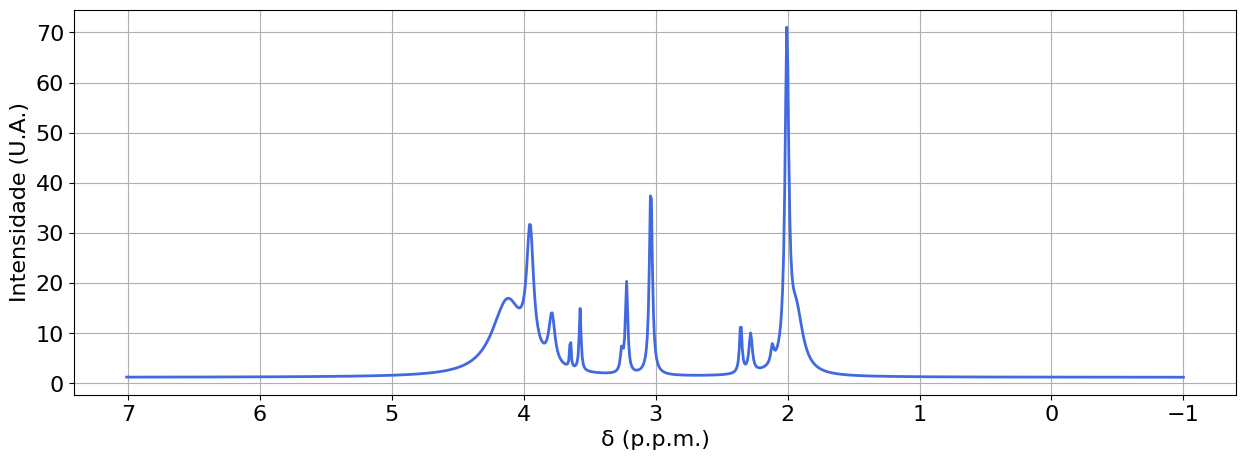
\includegraphics[scale=0.5]{sinal-de-controle.png}
    \centering
    \caption{Sinal de controle gerado para caracterização das variáveis.}
    \label{fig:1}
\end{figure}

\subsubsection{Sinal de controle de pico único} \label{sec:sinal-unico}

Além de averiguar a influência dos parâmetros tradicionais no processo do algoritmo, foi também verificada a necessidade de avaliar o 
comportamento dos parâmetros resultantes do processo, $S_0$, $\phi$, $\omega$ e $T_2$, com relação à qualidade do sinal, traduzida pela
sua relação sinal-ruído (do inglês, \textit{Signal-to-Noise Ratio}, SNR). Para prosseguir, foi escolhido um novo sinal de controle: a 
simulação de MRS de um único metabólito, o N-Acetylaspartato, ou NAA, escolhido por ser o maior pico dentre os metabólitos comumente 
encontrados no cérebro. Essa escolha foi motivada pela simplificação apresentada, visto que um único pico facilitaria o processo de 
investigação de possíveis fenômenos associados à distorções causada pela presença de ruído. A simulação foi feita com as mesmas 
condições de contorno apresentadas na \autoref{sec:sinal-completo}, podendo ser conferida pela \autoref{fig:2}.

\begin{figure} [H]
    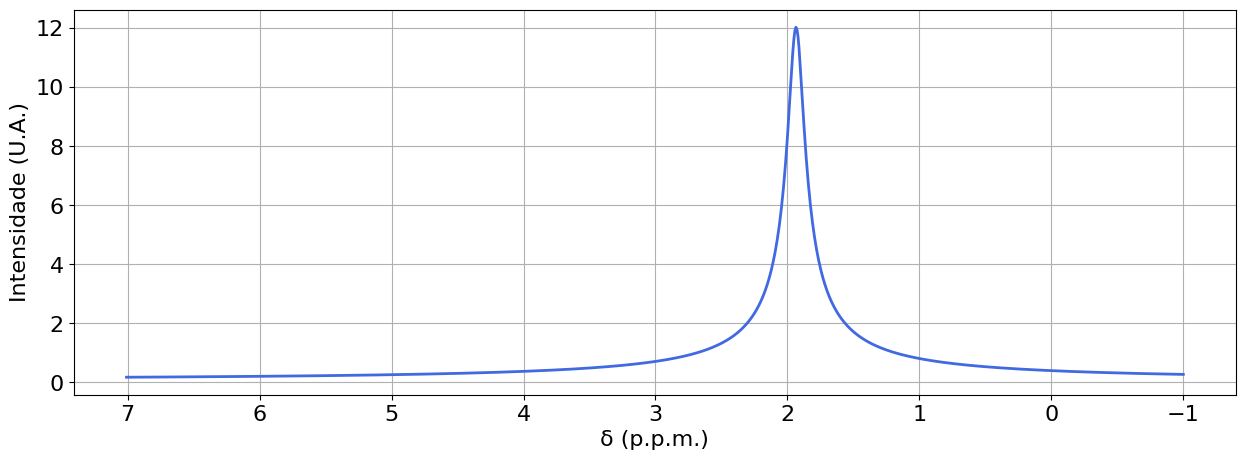
\includegraphics[scale=0.5]{sinal-unico-pico.png}
    \centering
    \caption{Sinal de controle de pico único gerado para estudo dos parâmetros resultantes.}
    \label{fig:2}
\end{figure}

\subsection{Corrupção dos Sinais}

A corrupção dos sinais foi realizada pela função \textit{awgn}, da biblioteca \textit{scikit-commpy}, uma biblioteca código aberto que 
reúne ferramentas para o estudo e simulação de sinais de comunicações. A função mencionada recebe como entrada o sinal e um valor de SNR, 
em dB, para o qual o sinal deve ter ao ser corrompido. A corrupção é feita com ruído gaussiano, diretamente no espectro do sinal, e usa 
a definição de $SNR$ explicada em \autoref{eq:26}.

\begin{equation} \label{eq:26}
    SNR = \frac{P_{sinal}}{P_{ruido}}
\end{equation}

Sendo $P_{sinal}$ e $P_{ruido}$ a potência média do sinal e a potência do ruído, respectivamente. 


\section{Resultados}

\subsection{Implementação do MPM}

O algoritmo foi implementado, assim como descrito na \autoref{sec:implement-mpm}, em etapas. Primeiro, foi testada a capacidade do mesmo 
de identificar exponencias decrescentes em condições ideias, a partir da implementação que não leva em conta ruído. A \autoref{fig:8} 
demonstra um exemplo, para o sinal descrito na \autoref{sec:sinal-completo}, de decomposição e reconstrução do mesmo a partir da implementação
que ignora a etapa que usa SVD, para $L$ de $40\%$. O algoritmo parece ter obtido sucesso na identificação dos picos dos metabólitos.

\begin{figure} [H]
    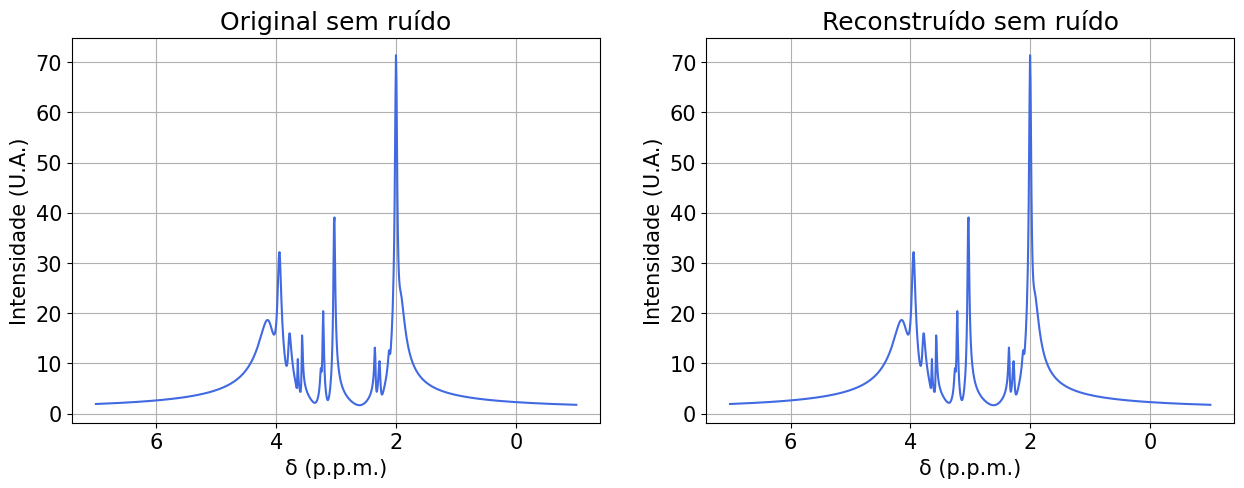
\includegraphics[scale=0.5]{mpm-sem-ruido.png}
    \centering
    \caption{Sinal limpo reconstruído a partir do processo de MPM sem ruído}
    \label{fig:8}
\end{figure}

Realizada a etapa de filtragem em um sinal sem ruído, foi implementada então a etapa da filtragem por SVD. Para testar seu funcionamento, o sinal
anteriormente usado foi corrompido com um SNR de valor $15 dB$. A \autoref{fig:9} demonstra um exemplo da decomposição e reconstrução desse sinal 
corrompido, para $L$ de $40\%$ e limite de ruído de $1^{-24}$. O limite de ruído foi escolhido extremamente baixo de maneira a testar se o algoritmo 
continuava a funcionar após implementação da etapa de SVD. 


\begin{figure} [H]
    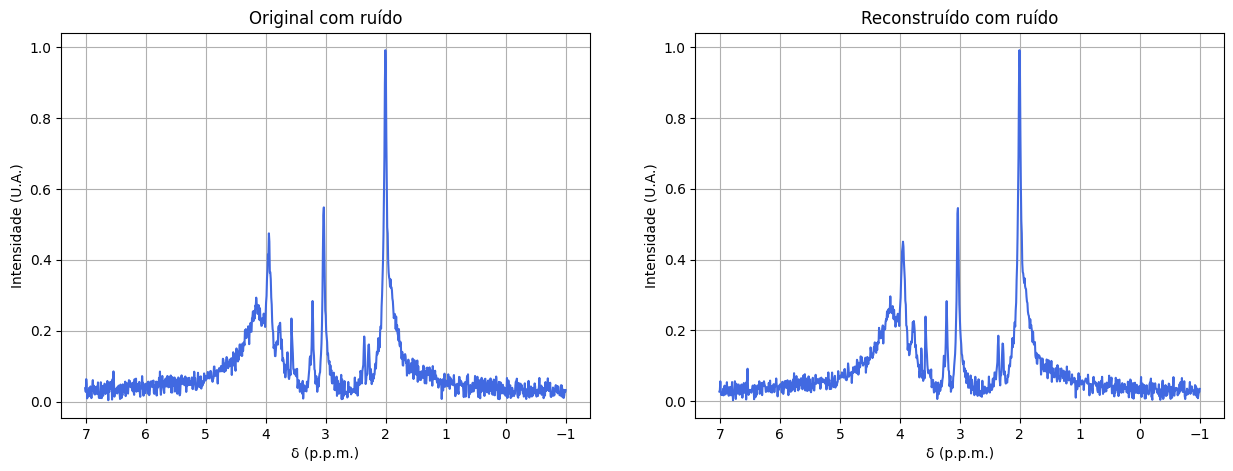
\includegraphics[scale=0.5]{mpm-com-ruido.png}
    \centering
    \caption{Sinal corrompido reconstruído a partir do processo de MPM com ruído de SNR equivalente a $15 dB$}
    \label{fig:9}
\end{figure}

\subsection{Separação de variáveis}

Para testar a capacidade de cálculo das variáveis $S_0$, $\phi$, $\omega$ e $T_2$ pelo programa, foi usado o sinal limpo descrito na \autoref{sec:sinal-unico}. 
Esse sinal foi processado pelo MPM no domínio do tempo, e a partir dos polos e resíduos calculados, teve suas variáveis resultantes calculadas. Todas essas 
variáveis, por sua vez, foram ordenadas em ordem crescente a partir da amplitude $S_0$.

\begin{figure} [H]
    \centering
    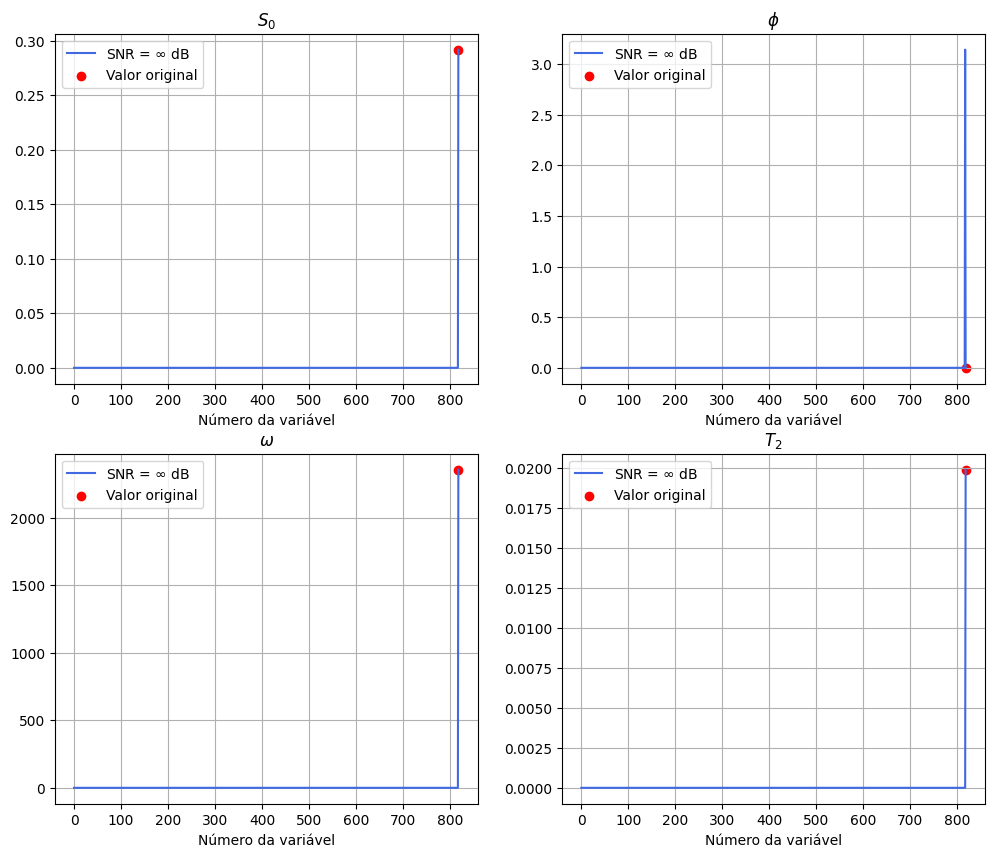
\includegraphics[scale=0.625]{var-0.png}
    \caption{Valor das variáveis para o sinal limpo}
    \label{fig:5}
\end{figure}

Como pode ser verificado pela \autoref{fig:5}, o cálculo foi realizado com sucesso, no qual todas as variáveis esperadas foram encontradas. É importante comentar 
que, por motivos de origem numérica, uma fase errônea de aproximadamente $\pi$ foi calculada, porém na reconstrução do sinal original, essa fase multiplica uma 
amplitude $S_0$ de valor 0, fazendo-a desaparecer. 

\subsection{Testagem de L sem ruído.}
Com a simulação e o algoritmo implementados com sucesso, foi possível enfim iniciar o estudo de seu comportamento na aplicação em sinais para 
diferentes parâmetros e processos, como inicialmente planejado. Como primeira etapa, foi testado para o algoritmo implementado como as variáveis resultantes do 
processo se comportavam com relação à variação de $L$, no sinal anteriormente apresentado, livre de ruído. Para isso, o algoritmo foi rodado 
com $L$ variando de $L_0 = 20\%$ do $N$ a $L_N = 80\%$ do $N$, limites além de $N/3$ e $N/2$ previamente estabelecidos, com o objetivo de verificar 
se havia alguma flutuação significativa nos valores das variáveis resultantes. Para cada $L$, variado nesse intervalo com um passo de $5\%$ do $N$ 
foram feitas 10 médias. O parâmetro $p$ foi fixado em 15, e a comparação foi feita por meio da 
Raiz do Erro Quadrático Médio (do inglês \textit{Root-mean-squared Error}, RMSE), podendo ser conferida pela \autoref{fig:3}.

\begin{figure} [H]
    \centering
    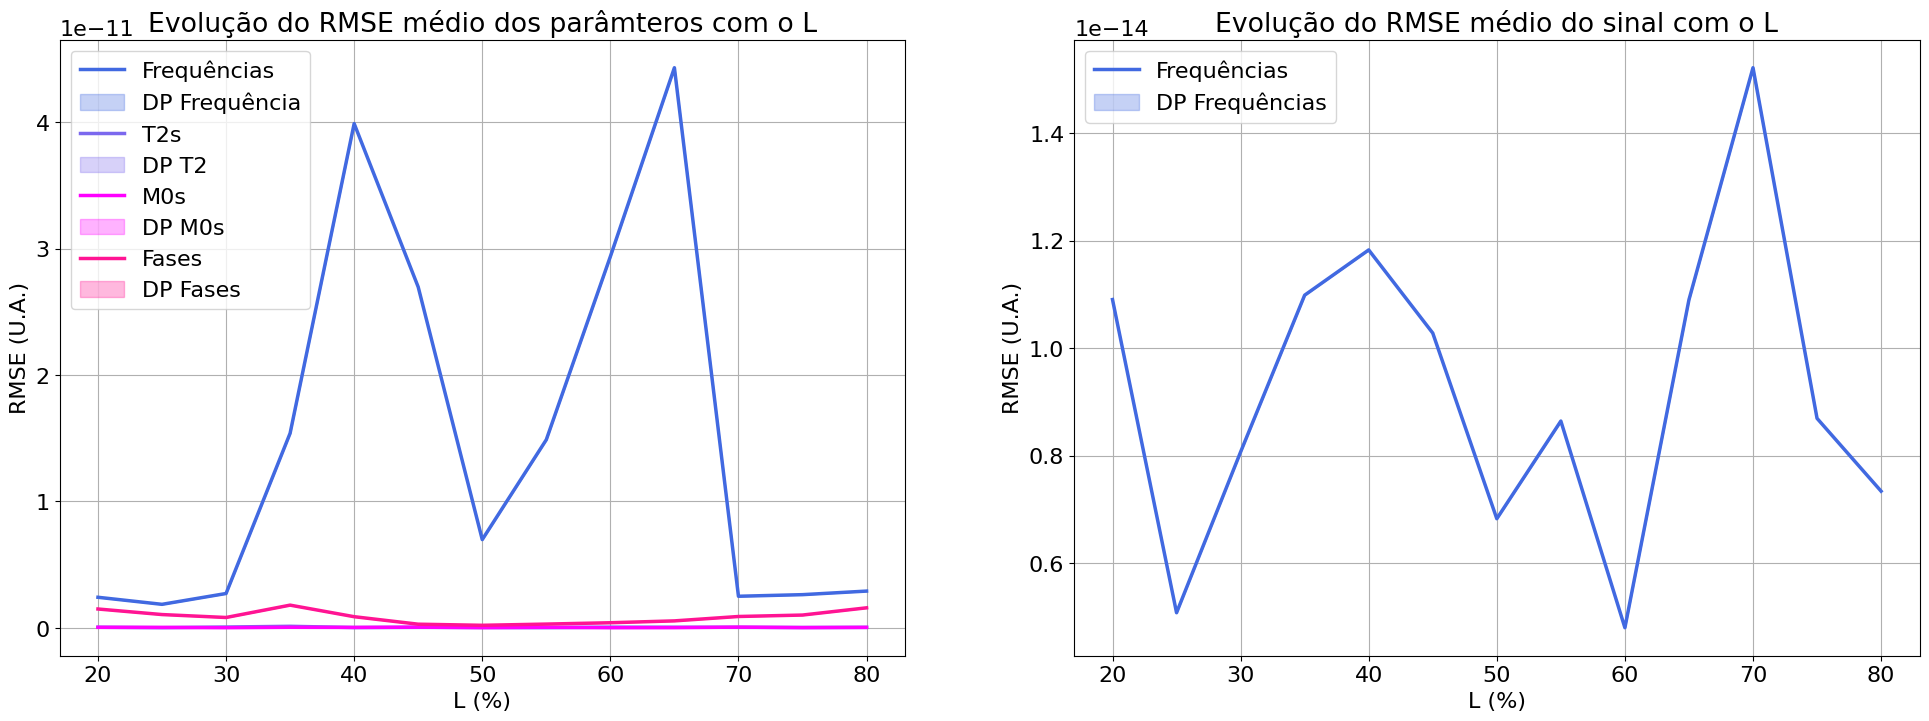
\includegraphics[scale=0.3125]{RMSE-L.png}
    \caption{Resultados para a variação de $L$}
    \label{fig:3}
\end{figure}

Pela \autoref{fig:3}, é possível concluir que a escolha do $L$ parece não impactar a capacidade de cálculo das variáveis originais do sinal 
limpo de ruído, visto que as flutuações de valor do RMSE médio são praticamente zero.

\subsection{Testagem de SVD sem ruído.}

Também foi testado, para o mesmo sinal, como as variáveis resultantes se comportavam com relação ao outro parâmetro do MPM, nesse caso, a 
ordem da variável de corte do SVD. $p$ foi variado entre $p_0 = 3$ e $p_N = 15$, com um passo de uma unidade, e $L = 40\%$. Para cada $p$, foram feitas 
também 10 médias. $p_0$ foi escolhido como 3 pois constatou-se que a partir de $p = 2$ os picos principais do sinal eram filtrados, impossibilitando a 
análise por meio do RMSE.

\begin{figure} [H]
    \centering
    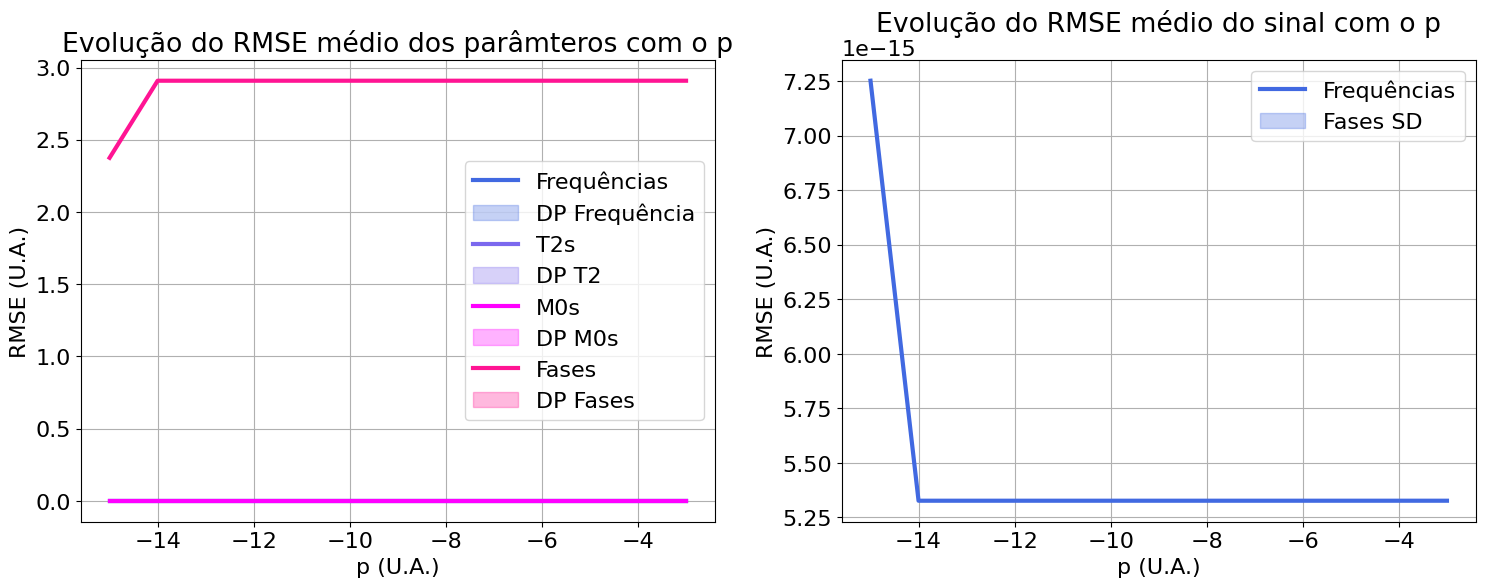
\includegraphics[scale=0.4166]{RMSE-p.png}
    \caption{Resultados para a variação de $p$}
    \label{fig:4}
\end{figure}

A priori, o evidente erro com relação às fases pode chamar a atenção, visto que a fase de entrada do sinal de controle era $\phi = 0$.
Constatou-se porém, após verificar manualmente os valores de fases gerados, que sua origem reside em pequenos erros numéricos que se propagam na função 
\textit{arctan2}, provocando um resultado de saída de aproximadamente $2\pi$ para fases calculadas, equivalente à fase esperada. Esclarecido esse 
importante detalhe, é possível concluir que, novamente para o sinal limpo, a $p$ não demonstra nenhuma influência significativa na capacidade de cálculo das 
variáveis originais.

\subsection{Relação entre as variáveis e o ruído}

Caracterizou-se o comportamento da variáveis anteriormente mencionadas com relação ao ruído, a simulação de pico único da \autoref{sec:sinal-unico} foi corrompida com
ruídos de diferentes níveis, variando o SNR resultante de $1.0$ a $100.0$. 

\begin{figure} [H]
    \centering
    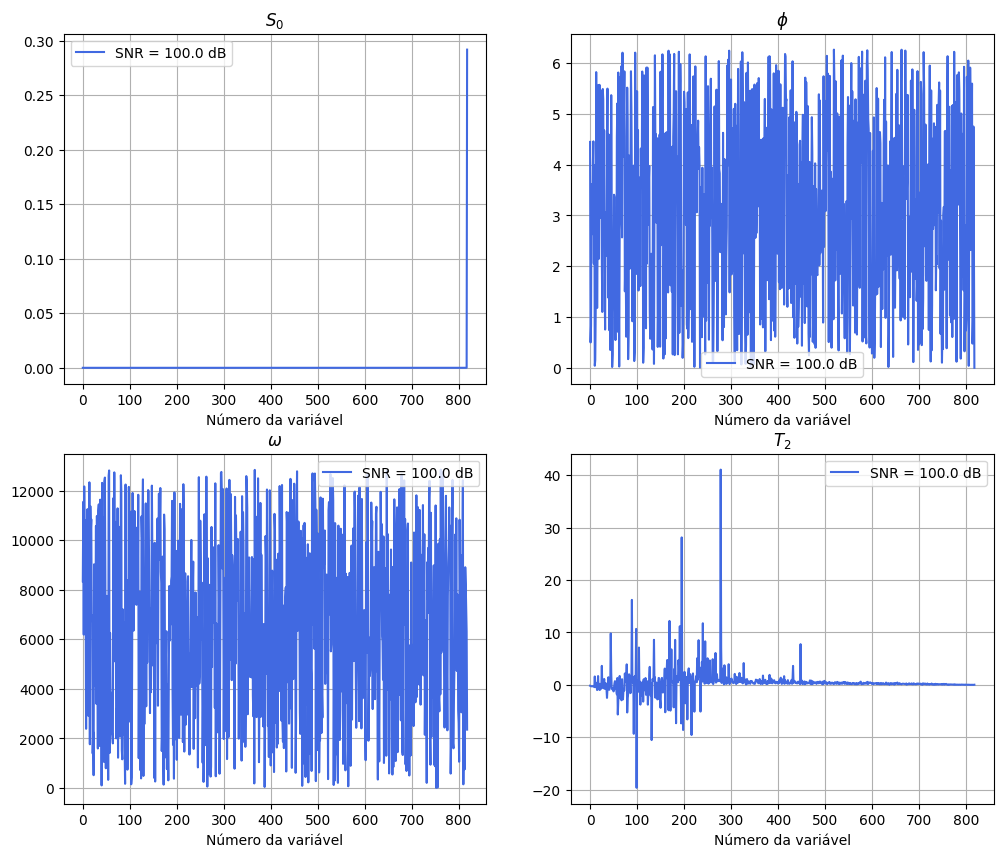
\includegraphics[scale=0.625]{var-1.png}
    \caption{Valor das variáveis para o segundo SNR, de valor $100$}
    \label{fig:6}
\end{figure}

Esse fenômeno de variáveis de valores "exóticos", presente no cálculo da fase em sinal limpo na \autoref{fig:5}, se mostrou comum ao longo dos outros processos de 
cálculo, tornando necessária a sua análise no contexto do algoritmo. Como pode ser verificado pela \autoref{fig:6}, para um valor de SNR mais baixo, nesse caso 100, 
o cálculo das frequência, tempos de decaimento e das fases demonstrou o mesmo comportamento anteriormente descrito, com valores oscilando de maneira ruidosa e pouco 
previsível, e amplitudes signficativas. Assim como descrito no caso de SNR infinito, a priori esse fenômeno pode se apresentar como obstáculo à capacidade de cálculo 
do MPM, porém novamente, quando analisada sob o contexto das outras variáveis, a maioria dos valores, quando multiplicados pela amplitude $S_0$, se anula.

\begin{figure} [H]
    \centering
    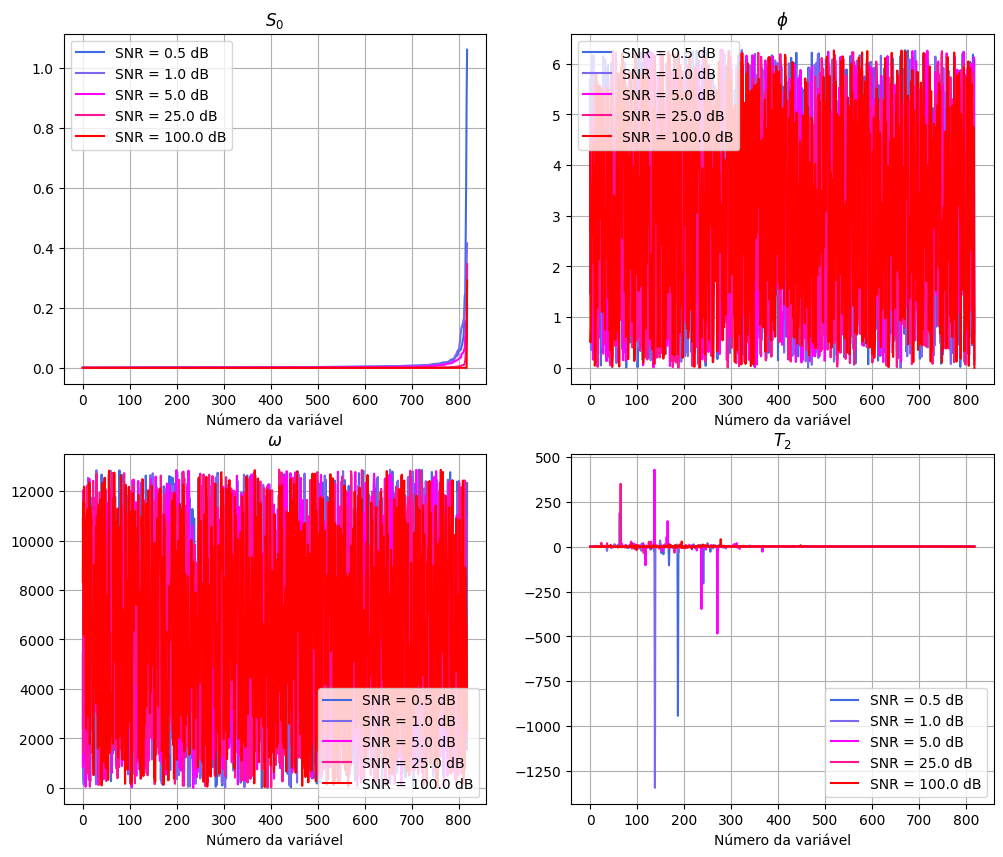
\includegraphics[scale=0.625]{vars-total.png}

    \caption{Valor das variáveis para o segundo SNR, de valor $100$}
    \label{fig:7}
\end{figure}

A variável $S_0$ aqui se mostra dominante para a construção do sinal final. Como verificado pela \autoref{fig:7}, conforme o SNR decresce, partindo da ordenação 
crescente de amplitudes, a distribuição de valores de $S_0$ não nulos aumenta. Esse aumento tanto em quantidade quanto em amplitude confere ao sinal final uma 
quantidade maior de frequências aparentemente aleatórias, compondo assim o ruído característico da corrupção originalmente aplicada.

\subsection{Relação entre picos e ruído}

Outra relação explorada por meio do MPM foi o comportamento das frequências do sinal original após serem corrompidas. Para isso, foi usado o sinal implementado em
\autoref{sec:sinal-unico}, de pico único, de maneira a simplificar a análise. Esse sinal foi corrompido com ruídos de SNRs resultantes no intervalo de 
$1.0$ a $100.0$, com passos não lineares. Cada sinal corrompido era desconstruído pelo MPM e tinha suas variáveis calculadas. Foi realizada então uma filtragem a 
partir do valor de seus picos $S_0$, na qual se calculava o maior pico, e a partir dele eram escolhidos os $n$ picos com valor maior ou igual a $5\%$ do maior pico. 
Esse procedimento foi realizado $50$ vezes para cada SNR, paara análise estatística.
 


 
\section{Conclusão}


\bibliographystyle{plain}
\bibliography{refs}


%nding the document
\end{document}